\documentclass[
	%a4paper, % Use A4 paper size
	letterpaper, % Use US letter paper size
]{jdf}

\usepackage{graphicx}
\usepackage{subfig}
\usepackage{float}

\author{
	Richard Albright \\
	903548616}
\email{ralbright7@gatech.edu}
\title{Project 3: Assess Learners}

\begin{document}
%\lsstyle

\maketitle

\begin{abstract}
The effect of leaf size on overfitting of various implementations of Classification and Regression Trees as measured by Root Mean Squared Error, $R^{2}$, and training time.
\end{abstract}

\section{Introduction}
This project analyzed the effect of leaf size on overfitting of various implementations of Classification and Regression Trees. The first experiment implemented a decision tree which found the best feature to split on by finding the feature that had the highest correlation with the output variable Y.  It then splits the dataset along the median value of that feature.  The second experiment implemented was a bagging learner using the decision tree from first experiment. The third experiment compares the decision tree from the prior two experiments with a random decision tree, where the dataset is split along the selection of a random feature.

\section{Methods}
An analysis of the above Classification and Regression Trees involved analyzing the effect of leaf size has on Root Mean Squared Error, $R^{2}$, and training time.  The Istanbul Stock Exchange Data Set was used to perform an in depth analysis of leaf size. The input variables (X) are the Istanbul stock exchange national 100 index, Standard \& Poor's 500 return index, Stock market return index of Germany, Stock market return index of UK, Stock market return index of Japan, Stock market return index of Brazil, and the MSCI European index. The predicted (Y) value was the MSCI emerging markets index.  The data set was split 60/40 into training (in sample) and test (out of sample
)sets. We then increased the leaf size of the decision trees from 1 through 50 using a step size of 1. The leaf size was then compared to the RMSE and $R^{2}$ statistics of both the in and out of sample sets. The training time of both the decision tree and random decision tree models were also compared.

\pagebreak

\section{Discussion}

\subsection{Experiment 1}

\begin{figure}[h]
	\begin{tabular}{c}
		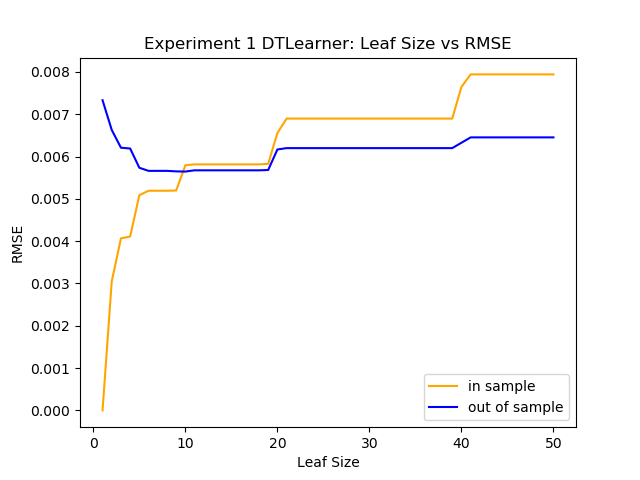
\includegraphics[height=10cm]{experiment_1.png} \\
		\textbf{Figure 1} \\
	\end{tabular}
\end{figure}

The first experiment analyzed the decision tree learner and compared its leaf size to RMSE for both in and out of sample sets.  Using the elbow method, overfitting occurs in the decision tree on leaf sizes <= 6. With a leaf size of one, we can perfectly predict the Y value for the in sample data as the RMSE = 0. While the out of sample RMSE = 0.0073. The RMSE of the in sample data is increasing as leaf size grows.  The RMSE of the out of sample data decreases until it reaches leaf size 6 at 0.0057, and then stabilizes out until leaf size 20 before starting to increase gradually as leaf size increases.

\pagebreak

\section{Experiment 2}

\begin{figure}[h]
	\begin{tabular}{c}
		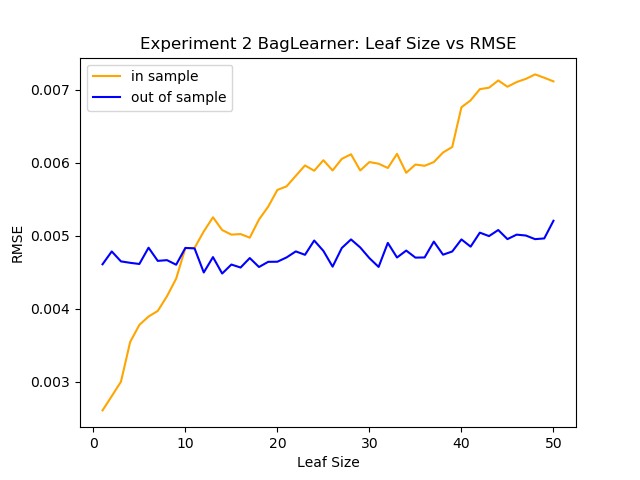
\includegraphics[height=10cm]{experiment_2.png} \\
		\textbf{Figure 2} \\
	\end{tabular}
\end{figure}

The second experiment used bagging of the decision tree from the first experiment.  20 bags were used with replacement.  The average prediction of those 20 bags was then returned for each leaf size. Bagging the decision tree reduces overfitting with respect to leaf size.  The out of sample RMSE drops from 0.0047 for leaf size 1, to 0.0046 for leaf size 6.  This is less than the RMSE decrease in Experiment 1, which dropped from 0.0073 to 0.0057 over the same range. The out of sample RMSE is no longer dropping significantly in Experiment 2 as leaf size increases.  Bagging will not eliminate overfitting completely as it's function is to reduce the variance over many runs.

\pagebreak

\section{Experiment 3}
\begin{figure}[h]
	\begin{tabular}{c}
		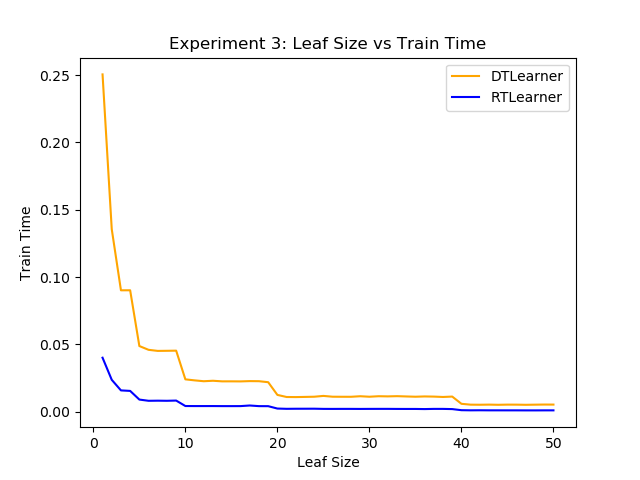
\includegraphics[height=10cm]{experiment_3a.png} \\
		\textbf{Figure 3} \\ 
	\end{tabular}
\end{figure}


The third experiment analyzes the effect of leaf size on training time for the decision tree used in Experiment 1, and a decision tree that is split on a random feature. As the leaf size drops, the training time for the random decision tree becomes significantly less than the decision tree used in Experiment 1.  This is because we are no longer checking all features for the highest absolute correlation before deciding which feature to split on, and we are just selecting a feature at random. The decision tree training time becomes exponentially worse than the random decision tree as leaf size drops below 10.

\pagebreak

\begin{figure}[h]
	\begin{tabular}{c}
		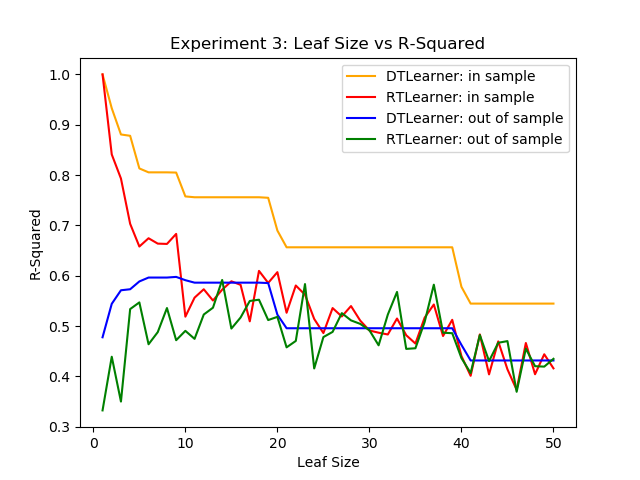
\includegraphics[height=10cm]{experiment_3b.png} \\
		\textbf{Figure 4} \\ 
	\end{tabular}
\end{figure}

The third experiment also analyzes the effect on leaf size on $R^{2}$ for the decision tree used in Experiment 1, and a decision tree that is split on a random feature. The decision tree plot lines are much smoother, as it is using the same feature for splitting for multiple nearby values of leaf size.  The random decision tree has more noise due to a different feature being selected for each leaf size.  Both models suffer from overfitting when leaf size is <= 6.  The original decision tree exhibits higher $R^{2}$ over the random decision tree model for all leaf sizes > 1 for the in sample set.  The original decision tree model performs better than the random decision tree model for leaf sizes <= 19 on the out of sample set.  For leaf sizes >=20, both models perform approximately the same, with the random decision tree model crossing over the original decision tree model's $R^{2}$ line due to its noise as explained above.  That being said, the original decision tree model is superior. The random decision tree model makes no attempts to split the data across meaningful features.

\section{Summary}
Overfitting can be reduced by conducting bagging on decision tree models.  With nominal differences in $R^{2}$ for leaf sizes >= 20, it would be interesting to see how bagging the random decision tree model performs vs the original bagging implementation on the decision tree model.  It could perform faster and still have acceptable accuracy.

\makeatletter
\renewcommand\@biblabel[1]{\textbullet}
\makeatother

\begin{thebibliography}{shortest-entry}

\bibitem{Wesner} Wesner, Janet \textit{MAE and RMSE — Which Metric is Better?}, https://medium.com/human-in-a-machine-world/mae-and-rmse-which-metric-is-better-e60ac3bde13d, 2016

\end{thebibliography}

\end{document}